\section{Evaluation}

In order to evaluate the performance of SFQ($D^2$) and compare it with
other schedulers, we implemented SFQ(D) and set up a benchmark
environment in a single cluster node, which has a hyperthreaded
quad-core 2.4GHz Intel processor, 24GB of RAM, and a 120G SATA SSD. 

The first step was to benchmark the SSD to determine the optimal
device latency and the expected depth parameter. 

\begin{figure}[t]
  \centering 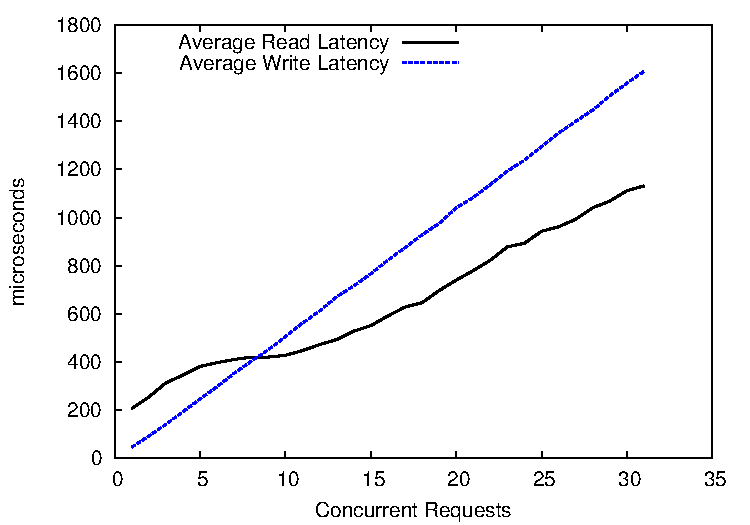
\includegraphics[width=\linewidth]{../../graphs/noop/latency_motivation.pdf}
  \caption{Average Latency vs IO depth}
  \label{fig:latMot}
\end{figure} 

\begin{figure}[t]
  \centering 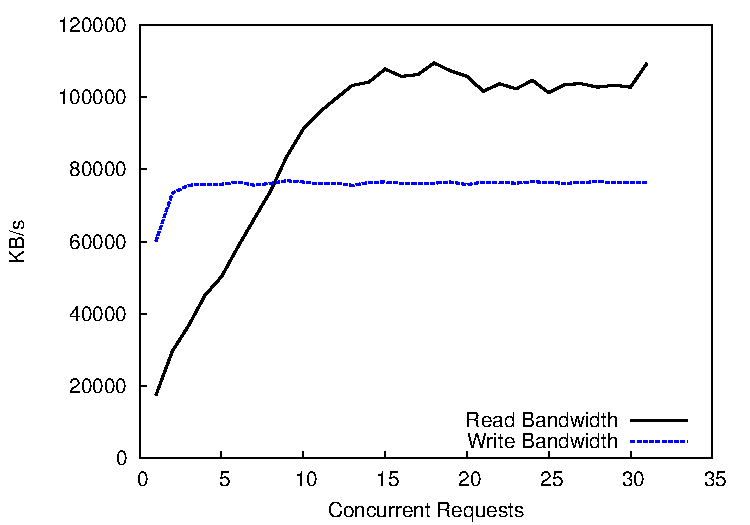
\includegraphics[width=\linewidth]{../../graphs/noop/bandwidth_motivation.pdf}
  \caption{Bandwidth vs IO depth}
  \label{fig:bandMot}
\end{figure}

%% We
%% tested different schedulers in different IO-depth and workloads. The
%% figure 1 and 2 showed the total latency and bandwidth results that two
%% process which have the same intensive level run concurrent. The figure
%% 3 and 4 showed that the results of concurrent running intensive write
%% and sparse read.\\

%% \begin{figure}[h!]
%%   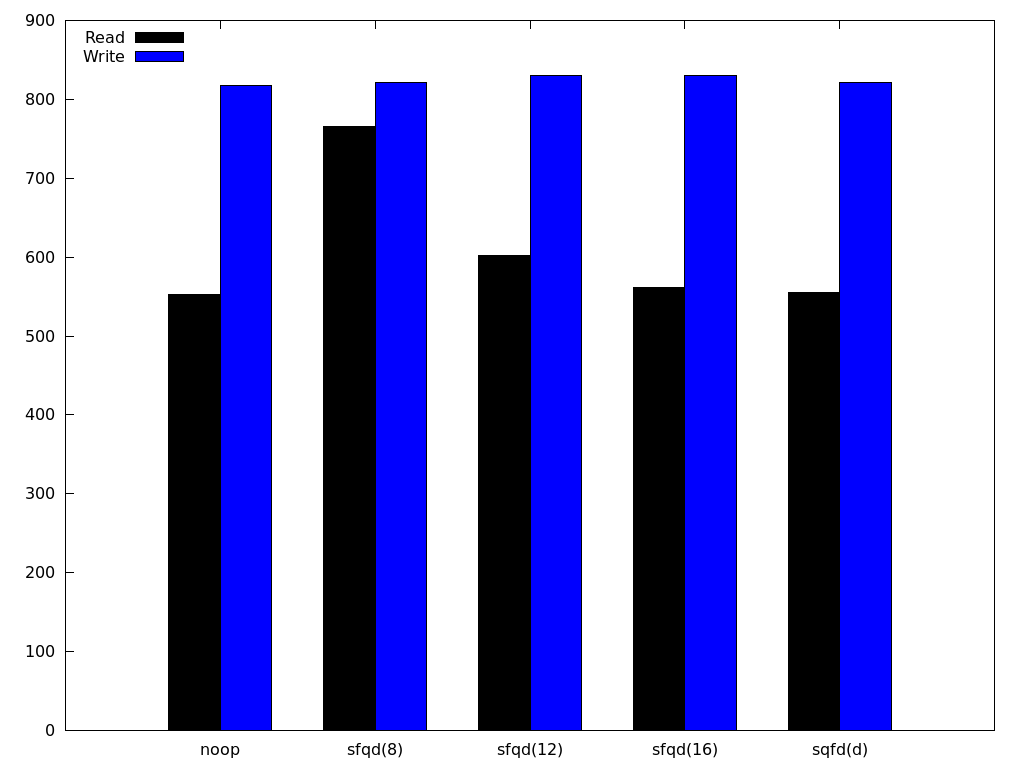
\includegraphics[width=1in,height=1in]{./image/lat_same}
%%   \centering
%%   \caption{Latency results in different schedulers}
%% \end{figure}
%% \begin{figure}[h!]
%%   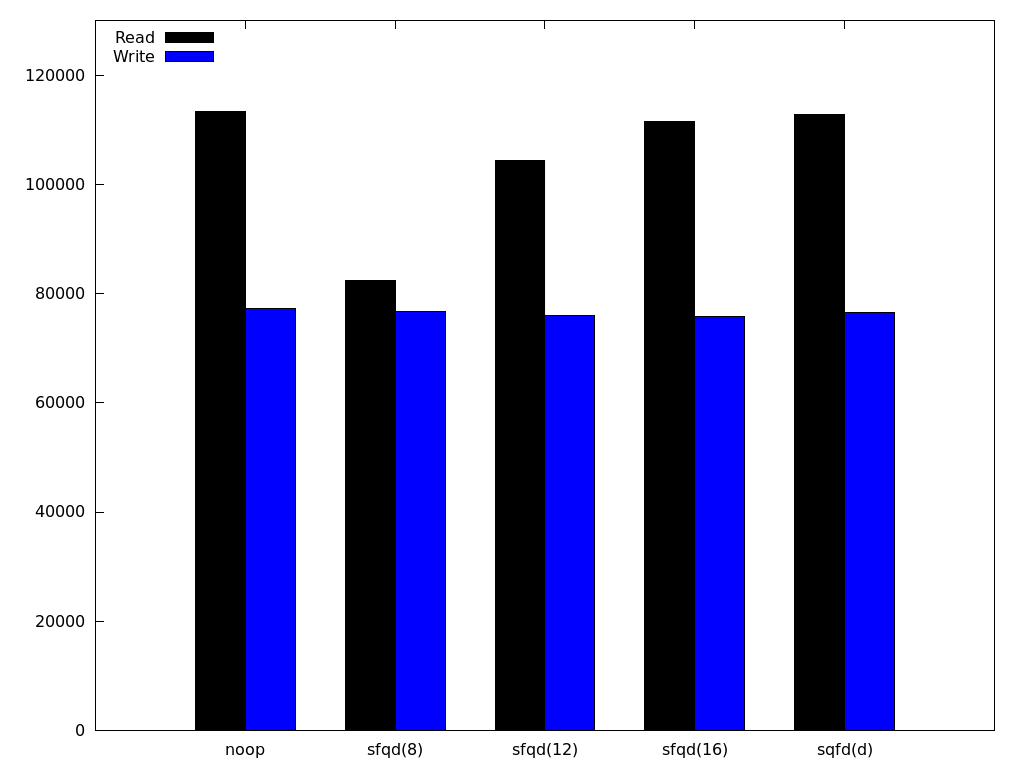
\includegraphics[width=1in,height=1in]{./image/bw_same}
%%   \centering
%%   \caption{bandwidth results in different schedulers}
%% \end{figure}

%% Figure 1 and 2 showed that the latency and bandwidth of SFQ($D^2$) are
%% better than the IO-depth is 8 and 12. And the performance of
%% SFQ($D^2$) is the same noop scheduler.\\


%% \begin{figure}[h!]
%%   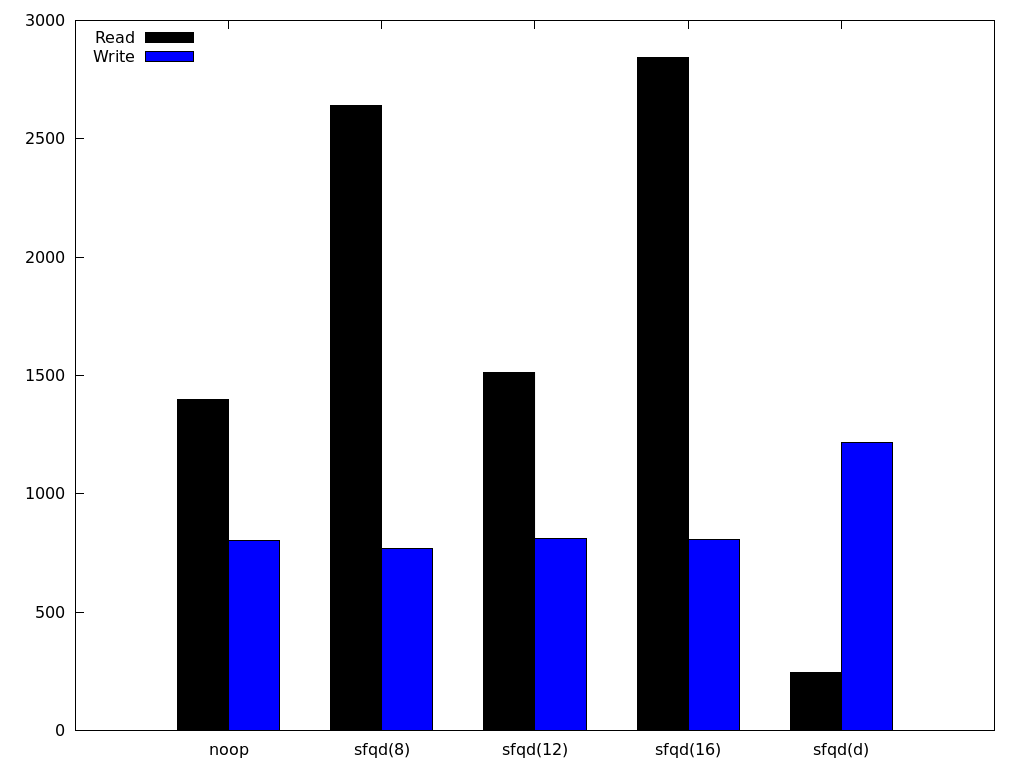
\includegraphics[width=1in,height=1in]{./image/lat_sparse}
%%   \centering
%%   \caption{Competing workloads latency results}
%% \end{figure}
%% \begin{figure}[h!]
%%   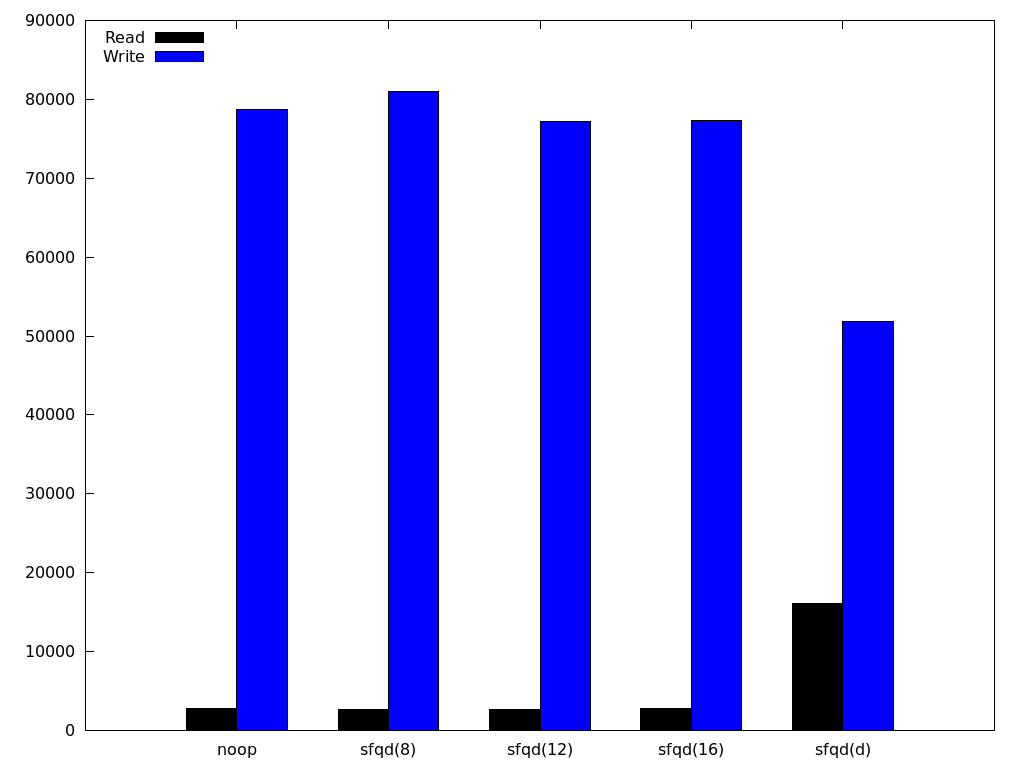
\includegraphics[width=1in,height=1in]{./image/bw_sparse}
%%   \centering
%%   \caption{Competing workloads bandwidth results}
%% \end{figure}

%% Figure 3 and 4 showed that the latency and bandwidth of SFQ($D^2$) are
%% much better than any other schedulers, although the write operation
%% performance is degrade 20 percentage due to they are sharing the same
%% device. Compare with noop and SFQD, SFQ($D^2$) can keep the fairness
%% better than others.\\
